\documentclass[12pt]{article}
\usepackage[english]{babel}
\usepackage[utf8x]{inputenc}
\usepackage{amsmath}
\usepackage{hyperref}
\usepackage{graphicx}
\usepackage{graphicx, lipsum,caption}
\usepackage[colorinlistoftodos]{todonotes}
\usepackage{caption}
\usepackage{subcaption}
\usepackage{framed}

\begin{document}
	
	\begin{titlepage}
		
		\newcommand{\HRule}{\rule{\linewidth}{0.5mm}} % Defines a new command for the horizontal lines, change thickness here
		
		\center % Center everything on the page
		
		%----------------------------------------------------------------------------------------
		%	HEADING SECTIONS
		%----------------------------------------------------------------------------------------
		
		\textsc{\LARGE Portland State University}\\[1.5cm] % Name of your university/college
		\textsc{\Large Deep Learning: Computational Structures and Programming}\\[0.5cm] % Major heading such as course name
		\textsc{\large Winter 2021}\\[0.5cm] % Minor heading such as course title
		
		%----------------------------------------------------------------------------------------
		%	TITLE SECTION
		%----------------------------------------------------------------------------------------
		
		\HRule \\[0.4cm]
		{ \huge \bfseries Project \#3}\\[0.4cm] % Title of your document
		\HRule \\[1.5cm]
		
		%----------------------------------------------------------------------------------------
		%	AUTHOR SECTION
		%----------------------------------------------------------------------------------------
		
		\begin{minipage}{0.4\textwidth}
			\begin{flushleft} \large
				\emph{Author:}\\
				Hermann \textsc{Yepdjio} % Your name
			\end{flushleft}
		\end{minipage}
		~
		\begin{minipage}{0.4\textwidth}
			\begin{flushright} \large
				\emph{Professor:} \\
				Dr. Suresh \textsc{Singh} % Supervisor's Name
			\end{flushright}
		\end{minipage}\\[1cm]
		
		% If you don't want a supervisor, uncomment the two lines below and remove the section above
		%\Large \emph{Author:}\\
		%John \textsc{Smith}\\[3cm] % Your name
		
		%----------------------------------------------------------------------------------------
		%	DATE SECTION
		%----------------------------------------------------------------------------------------
		
		{\large \today}\\[0.7cm] % Date, change the \today to a set date if you want to be precise
		
		%----------------------------------------------------------------------------------------
		%	LOGO SECTION
		%----------------------------------------------------------------------------------------
		
		
\includegraphics[width=7cm]{PSU_LOGO.png}\\[.5cm] % Include a department/university logo - this will require the graphicx package
		
		%----------------------------------------------------------------------------------------
		
		\vfill % Fill the rest of the page with whitespace
		
	\end{titlepage}
	%\newpage
	%\tableofcontents
	\newpage
	
	
	
	\section{Transfer Learning Using ResNet\_18}
		\subsection{Visualize a Few Images}
		
			\begin{figure}[h]
				\centering
				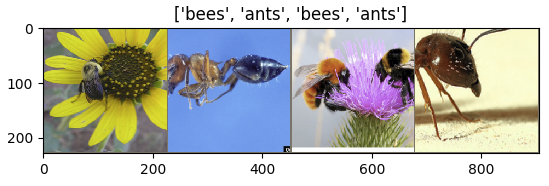
\includegraphics[width=12cm]{Figure_1.png}
				\label{fig:sub1}
			\end{figure}
		
		\subsection{Train and Test Results}
			\begin{figure}[h]
				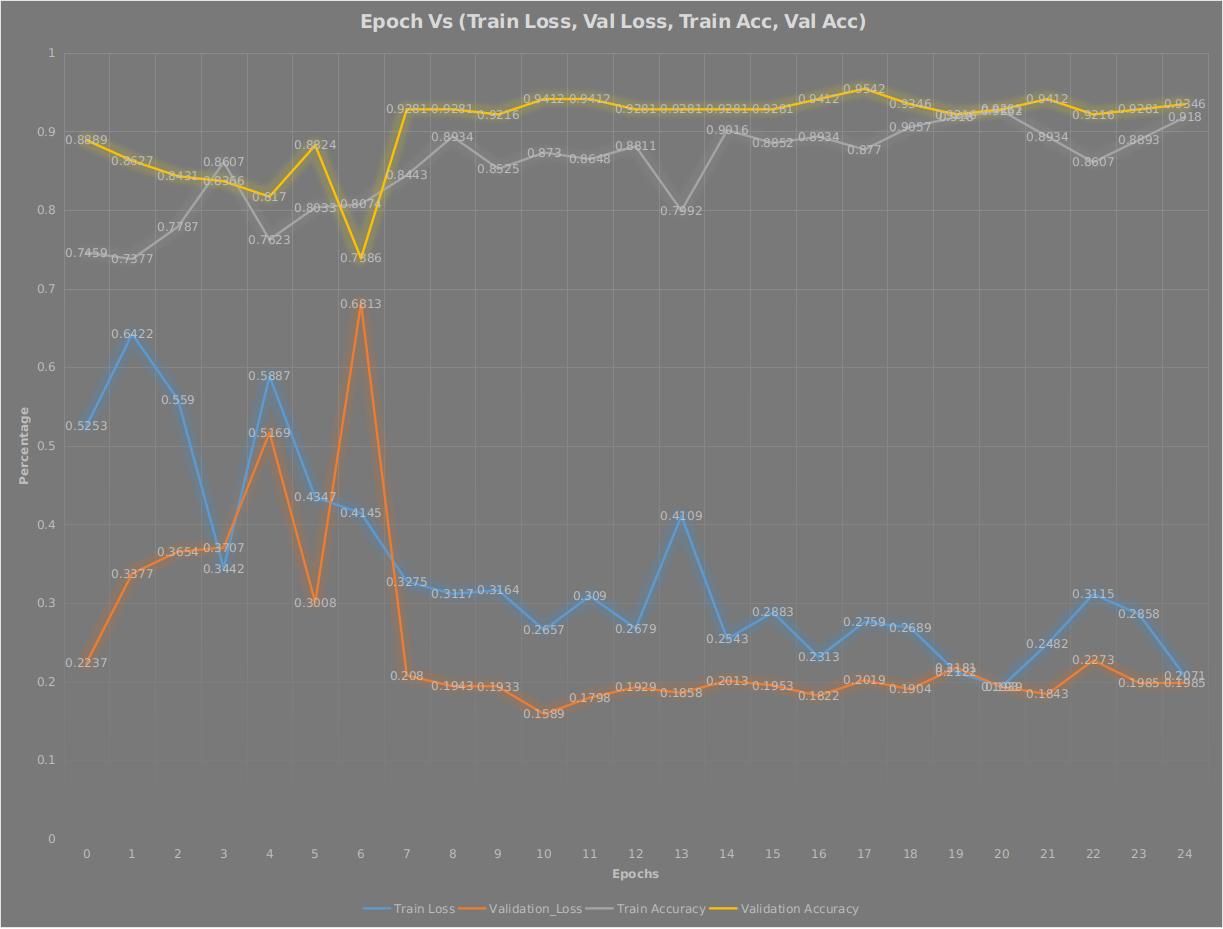
\includegraphics[width=13cm]{Plot_1.png}
				\captionsetup{justification=centering,margin=1cm}
				\label{fig:sub1}
			\end{figure}
		
			\begin{table}[h]
			\centering
			\label{tab:my-table}
			\resizebox{8cm}{!}{%
			\begin{tabular}{lcccc}
				\hline
				Epoch & Train Loss & Validation\_Loss & Train Accuracy & Validation Accuracy \\ \hline
				0     & 0.5253     & 0.2237           & 0.7459         & 0.8889              \\
				1     & 0.6422     & 0.3377           & 0.7377         & 0.8627              \\
				2     & 0.559      & 0.3654           & 0.7787         & 0.8431              \\
				3     & 0.3442     & 0.3707           & 0.8607         & 0.8366              \\
				4     & 0.5887     & 0.5169           & 0.7623         & 0.817               \\
				5     & 0.4347     & 0.3008           & 0.8033         & 0.8824              \\
				6     & 0.4145     & 0.6813           & 0.8074         & 0.7386              \\
				7     & 0.3275     & 0.208            & 0.8443         & 0.9281              \\
				8     & 0.3117     & 0.1943           & 0.8934         & 0.9281              \\
				9     & 0.3164     & 0.1933           & 0.8525         & 0.9216              \\
				10    & 0.2657     & 0.1589           & 0.873          & 0.9412              \\
				11    & 0.309      & 0.1798           & 0.8648         & 0.9412              \\
				12    & 0.2679     & 0.1929           & 0.8811         & 0.9281              \\
				13    & 0.4109     & 0.1858           & 0.7992         & 0.9281              \\
				14    & 0.2543     & 0.2013           & 0.9016         & 0.9281              \\
				15    & 0.2883     & 0.1953           & 0.8852         & 0.9281              \\
				16    & 0.2313     & 0.1822           & 0.8934         & 0.9412              \\
				17    & 0.2759     & 0.2019           & 0.877          & 0.9542              \\
				18    & 0.2689     & 0.1904           & 0.9057         & 0.9346              \\
				19    & 0.2122     & 0.2181           & 0.918          & 0.9216              \\
				20    & 0.1939     & 0.193            & 0.9262         & 0.9281              \\
				21    & 0.2482     & 0.1843           & 0.8934         & 0.9412              \\
				22    & 0.3115     & 0.2273           & 0.8607         & 0.9216              \\
				23    & 0.2858     & 0.1985           & 0.8893         & 0.9281              \\
				24    & 0.2071     & 0.1985           & 0.918          & 0.9346              \\ \hline
			\end{tabular}
		}
		\end{table}
		
		\subsection{Visualize the Model}
		
			\begin{figure}[h]
				\centering
				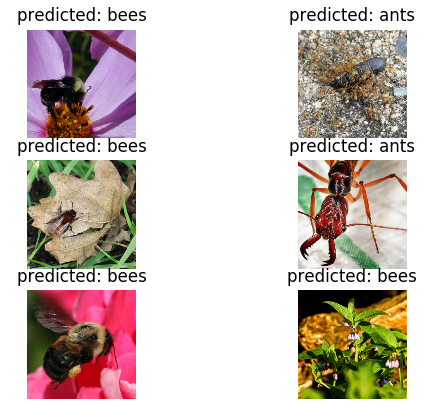
\includegraphics[width=7cm]{Figure_2.png}
				\label{fig:sub1}
			\end{figure}
		\newpage
		\subsection{ConvNet as Fixed Feature Extractor: Train and Test Results}
		
			\begin{figure}[h]
				\centering
				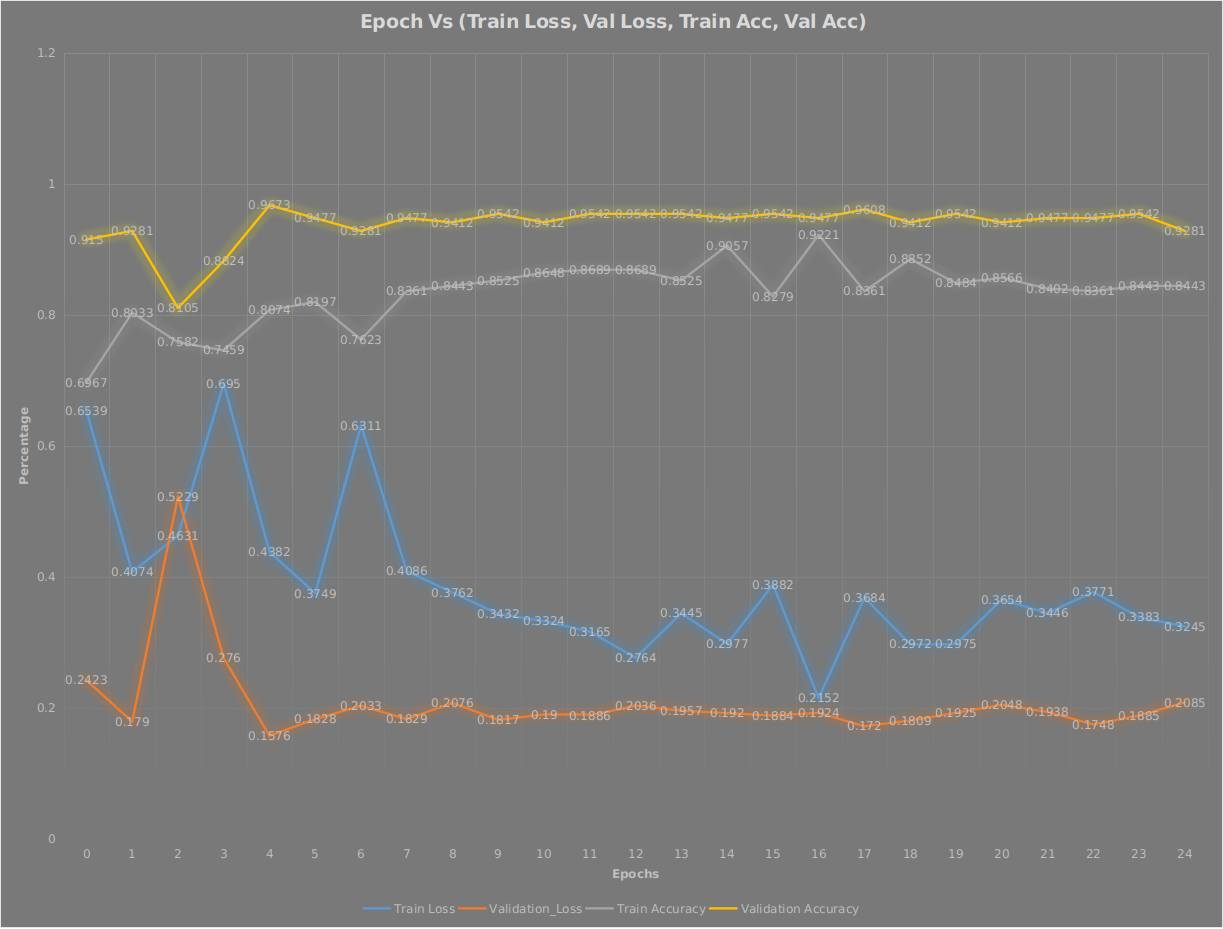
\includegraphics[width=13cm]{Plot_2.png}
				\label{fig:sub1}
			\end{figure}
		
		\newpage
			\begin{table}[h]
				\centering
				\label{tab:my-table}
			\resizebox{8cm}{!}{%
				\begin{tabular}{lcccc}
					\hline
					Epoch & Train Loss & Validation\_Loss & Train Accuracy & Validation Accuracy \\ \hline
					0     & 0.6539     & 0.2423           & 0.6967         & 0.915               \\
					1     & 0.4074     & 0.179            & 0.8033         & 0.9281              \\
					2     & 0.4631     & 0.5229           & 0.7582         & 0.8105              \\
					3     & 0.695      & 0.276            & 0.7459         & 0.8824              \\
					4     & 0.4382     & 0.1576           & 0.8074         & 0.9673              \\
					5     & 0.3749     & 0.1828           & 0.8197         & 0.9477              \\
					6     & 0.6311     & 0.2033           & 0.7623         & 0.9281              \\
					7     & 0.4086     & 0.1829           & 0.8361         & 0.9477              \\
					8     & 0.3762     & 0.2076           & 0.8443         & 0.9412              \\
					9     & 0.3432     & 0.1817           & 0.8525         & 0.9542              \\
					10    & 0.3324     & 0.19             & 0.8648         & 0.9412              \\
					11    & 0.3165     & 0.1886           & 0.8689         & 0.9542              \\
					12    & 0.2764     & 0.2036           & 0.8689         & 0.9542              \\
					13    & 0.3445     & 0.1957           & 0.8525         & 0.9542              \\
					14    & 0.2977     & 0.192            & 0.9057         & 0.9477              \\
					15    & 0.3882     & 0.1884           & 0.8279         & 0.9542              \\
					16    & 0.2152     & 0.1924           & 0.9221         & 0.9477              \\
					17    & 0.3684     & 0.172            & 0.8361         & 0.9608              \\
					18    & 0.2972     & 0.1809           & 0.8852         & 0.9412              \\
					19    & 0.2975     & 0.1925           & 0.8484         & 0.9542              \\
					20    & 0.3654     & 0.2048           & 0.8566         & 0.9412              \\
					21    & 0.3446     & 0.1938           & 0.8402         & 0.9477              \\
					22    & 0.3771     & 0.1748           & 0.8361         & 0.9477              \\
					23    & 0.3383     & 0.1885           & 0.8443         & 0.9542              \\
					24    & 0.3245     & 0.2085           & 0.8443         & 0.9281              \\ \hline
				\end{tabular}
			}
			\end{table}
		
		
		\subsection{ConvNet as Fixed Feature Extractor: Visualize the Model}
		
			\begin{figure}[h]
				\centering
				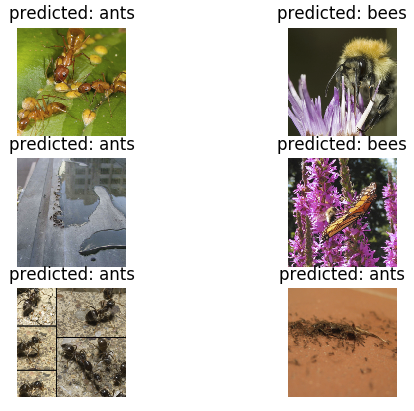
\includegraphics[width=6cm]{Figure_3.png}
				\captionsetup{justification=centering,margin=1cm}
				\label{fig:sub1}
			\end{figure}
		
	\newpage
	
	
	\section{Transfer Learning Using GoogleNet}
	\subsection{Visualize a Few Images}
	
	\begin{figure}[h]
		\centering
		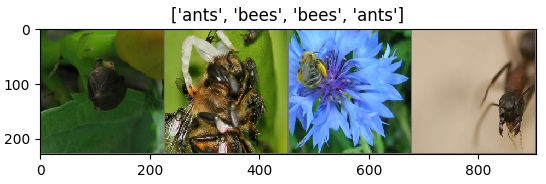
\includegraphics[width=12cm]{Figure_4.png}
		\label{fig:sub1}
	\end{figure}
	
	\subsection{Train and Test Results}
	\begin{figure}[h]
		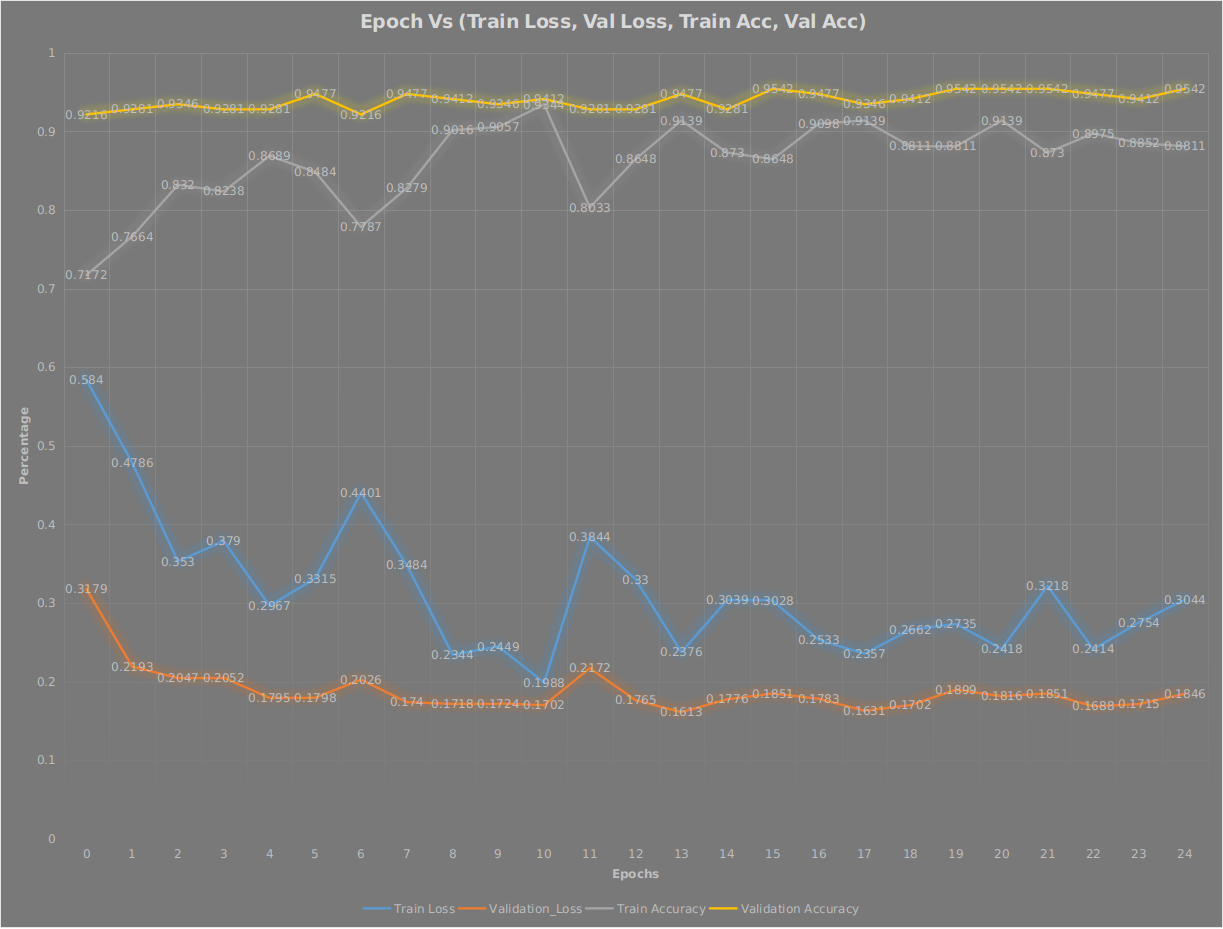
\includegraphics[width=13cm]{Plot_3.png}
		\captionsetup{justification=centering,margin=1cm}
		\label{fig:sub1}
	\end{figure}
	
	\begin{table}[h]
		\centering
		\label{tab:my-table}
		\resizebox{8cm}{!}{%
			\begin{tabular}{lcccc}
				\hline
				Epoch & Train Loss & Validation\_Loss & Train Accuracy & Validation Accuracy \\ \hline
				0     & 0.584      & 0.3179           & 0.7172         & 0.9216              \\
				1     & 0.4786     & 0.2193           & 0.7664         & 0.9281              \\
				2     & 0.353      & 0.2047           & 0.832          & 0.9346              \\
				3     & 0.379      & 0.2052           & 0.8238         & 0.9281              \\
				4     & 0.2967     & 0.1795           & 0.8689         & 0.9281              \\
				5     & 0.3315     & 0.1798           & 0.8484         & 0.9477              \\
				6     & 0.4401     & 0.2026           & 0.7787         & 0.9216              \\
				7     & 0.3484     & 0.174            & 0.8279         & 0.9477              \\
				8     & 0.2344     & 0.1718           & 0.9016         & 0.9412              \\
				9     & 0.2449     & 0.1724           & 0.9057         & 0.9346              \\
				10    & 0.1988     & 0.1702           & 0.9344         & 0.9412              \\
				11    & 0.3844     & 0.2172           & 0.8033         & 0.9281              \\
				12    & 0.33       & 0.1765           & 0.8648         & 0.9281              \\
				13    & 0.2376     & 0.1613           & 0.9139         & 0.9477              \\
				14    & 0.3039     & 0.1776           & 0.873          & 0.9281              \\
				15    & 0.3028     & 0.1851           & 0.8648         & 0.9542              \\
				16    & 0.2533     & 0.1783           & 0.9098         & 0.9477              \\
				17    & 0.2357     & 0.1631           & 0.9139         & 0.9346              \\
				18    & 0.2662     & 0.1702           & 0.8811         & 0.9412              \\
				19    & 0.2735     & 0.1899           & 0.8811         & 0.9542              \\
				20    & 0.2418     & 0.1816           & 0.9139         & 0.9542              \\
				21    & 0.3218     & 0.1851           & 0.873          & 0.9542              \\
				22    & 0.2414     & 0.1688           & 0.8975         & 0.9477              \\
				23    & 0.2754     & 0.1715           & 0.8852         & 0.9412              \\
				24    & 0.3044     & 0.1846           & 0.8811         & 0.9542              \\ \hline
			\end{tabular}
		}
	\end{table}
	
	\subsection{Visualize the Model}
	
	\begin{figure}[h]
		\centering
		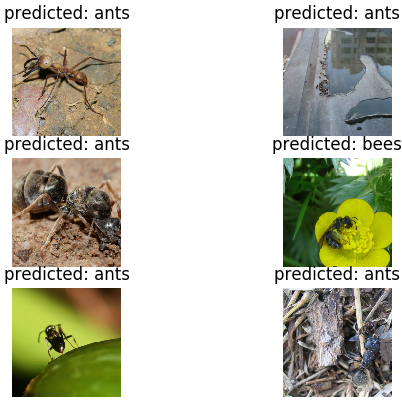
\includegraphics[width=6cm]{Figure_5.png}
		\label{fig:sub1}
	\end{figure}
	\newpage
	\subsection{ConvNet as Fixed Feature Extractor: Train and Test Results}
	
	\begin{figure}[h]
		\centering
		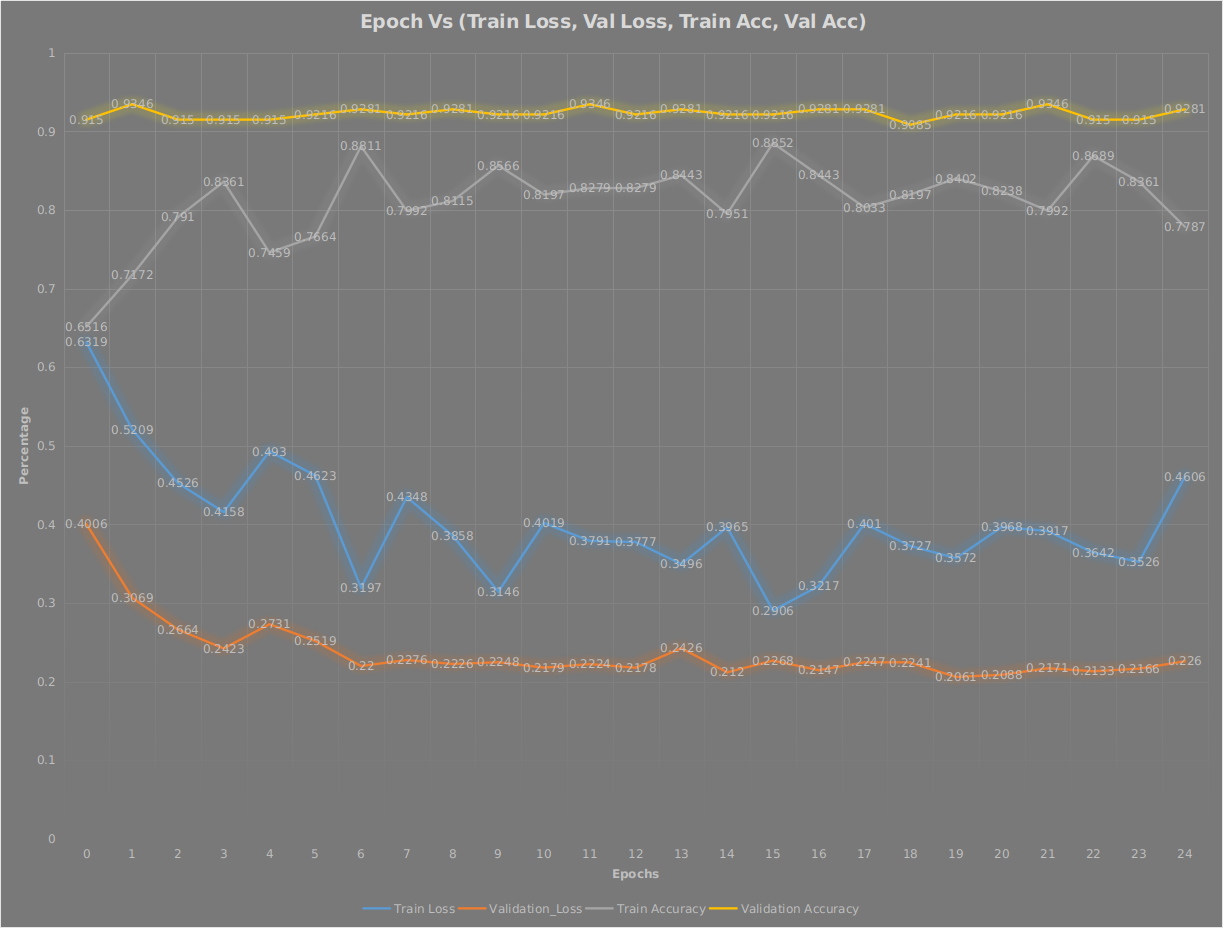
\includegraphics[width=13cm]{Plot_4.png}
		\label{fig:sub1}
	\end{figure}
	
	\newpage
	\begin{table}[h]
		\centering
		\label{tab:my-table}
		\resizebox{8cm}{!}{%
			\begin{tabular}{lcccc}
				\hline
				Epoch & Train Loss & Validation\_Loss & Train Accuracy & Validation Accuracy \\ \hline
				0     & 0.6319     & 0.4006           & 0.6516         & 0.915               \\
				1     & 0.5209     & 0.3069           & 0.7172         & 0.9346              \\
				2     & 0.4526     & 0.2664           & 0.791          & 0.915               \\
				3     & 0.4158     & 0.2423           & 0.8361         & 0.915               \\
				4     & 0.493      & 0.2731           & 0.7459         & 0.915               \\
				5     & 0.4623     & 0.2519           & 0.7664         & 0.9216              \\
				6     & 0.3197     & 0.22             & 0.8811         & 0.9281              \\
				7     & 0.4348     & 0.2276           & 0.7992         & 0.9216              \\
				8     & 0.3858     & 0.2226           & 0.8115         & 0.9281              \\
				9     & 0.3146     & 0.2248           & 0.8566         & 0.9216              \\
				10    & 0.4019     & 0.2179           & 0.8197         & 0.9216              \\
				11    & 0.3791     & 0.2224           & 0.8279         & 0.9346              \\
				12    & 0.3777     & 0.2178           & 0.8279         & 0.9216              \\
				13    & 0.3496     & 0.2426           & 0.8443         & 0.9281              \\
				14    & 0.3965     & 0.212            & 0.7951         & 0.9216              \\
				15    & 0.2906     & 0.2268           & 0.8852         & 0.9216              \\
				16    & 0.3217     & 0.2147           & 0.8443         & 0.9281              \\
				17    & 0.401      & 0.2247           & 0.8033         & 0.9281              \\
				18    & 0.3727     & 0.2241           & 0.8197         & 0.9085              \\
				19    & 0.3572     & 0.2061           & 0.8402         & 0.9216              \\
				20    & 0.3968     & 0.2088           & 0.8238         & 0.9216              \\
				21    & 0.3917     & 0.2171           & 0.7992         & 0.9346              \\
				22    & 0.3642     & 0.2133           & 0.8689         & 0.915               \\
				23    & 0.3526     & 0.2166           & 0.8361         & 0.915               \\
				24    & 0.4606     & 0.226            & 0.7787         & 0.9281              \\ \hline
			\end{tabular}
		}
	\end{table}
	
	
	\subsection{ConvNet as Fixed Feature Extractor: Visualize the Model}
	
	\begin{figure}[h]
		\centering
		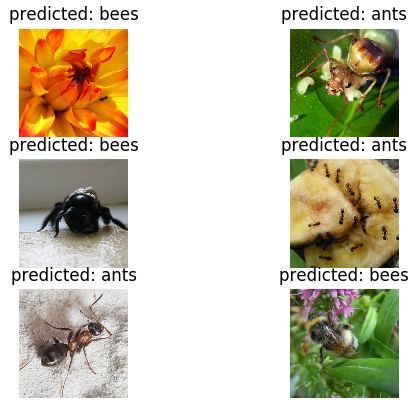
\includegraphics[width=6cm]{Figure_6.png}
		\captionsetup{justification=centering,margin=1cm}
		\label{fig:sub1}
	\end{figure}

	\newpage
	
	\section{Comparison Between ResNet and GoogleNet}
	
	\begin{itemize}
		\item GoogleNet takes more time to train then ResNet (11m59s vs 10m37s for the first experiment and 6m26s vs 4m34s for the second experiment) though it has less parameters (GoogleNet (V1) has about 5 million parameters vs about 11 million parameters for ResNet18). The reason to this is that ResNet has identity shortcut connections that allow to skip some of the layers when necessary during training in order to get rid of the vanishing gradient problem. Doing this also considerably reduces the complexity of the network, allowing faster training.
		\item ResNet seems to produce better classification results than GoogleNet (95.42\% vs 95.42\% for the first experiment and 96.76\% vs 93.46\% for the second experiment). The reason to this is that ResNet has more parameters than GoogleNet, which in theory means that the former should be able to make better predictions than the latter at the condition of finding a way to deal with the vanishing gradient problem. The residual blocks in ResNet allow the network to deal with the vanishing gradient problem while keeping a good performance.  
	\end{itemize}
		
		
	%\bibliographystyle{ieeetr}
	%\bibliography{references}
	
\end{document}
